
% bare_conf.tex
% V1.3
% 2007/01/11
% by Michael Shell
% See:
% http://www.michaelshell.org/
% for current contact information.
%
% This is a skeleton file demonstrating the use of IEEEtran.cls
% (requires IEEEtran.cls version 1.7 or later) with an IEEE conference paper.
%
% Support sites:
% http://www.michaelshell.org/tex/ieeetran/
% http://www.ctan.org/tex-archive/macros/latex/contrib/IEEEtran/
% and
% http://www.ieee.org/

%*************************************************************************
% Legal Notice:
% This code is offered as-is without any warranty either expressed or
% implied; without even the implied warranty of MERCHANTABILITY or
% FITNESS FOR A PARTICULAR PURPOSE! 
% User assumes all risk.
% In no event shall IEEE or any contributor to this code be liable for
% any damages or losses, including, but not limited to, incidental,
% consequential, or any other damages, resulting from the use or misuse
% of any information contained here.
%
% All comments are the opinions of their respective authors and are not
% necessarily endorsed by the IEEE.
%
% This work is distributed under the LaTeX Project Public License (LPPL)
% ( http://www.latex-project.org/ ) version 1.3, and may be freely used,
% distributed and modified. A copy of the LPPL, version 1.3, is included
% in the base LaTeX documentation of all distributions of LaTeX released
% 2003/12/01 or later.
% Retain all contribution notices and credits.
% ** Modified files should be clearly indicated as such, including  **
% ** renaming them and changing author support contact information. **
%
% File list of work: IEEEtran.cls, IEEEtran_HOWTO.pdf, bare_adv.tex,
%                    bare_conf.tex, bare_jrnl.tex, bare_jrnl_compsoc.tex
%*************************************************************************

% *** Authors should verify (and, if needed, correct) their LaTeX system  ***
% *** with the testflow diagnostic prior to trusting their LaTeX platform ***
% *** with production work. IEEE's font choices can trigger bugs that do  ***
% *** not appear when using other class files.                            ***
% The testflow support page is at:
% http://www.michaelshell.org/tex/testflow/



% Note that the a4paper option is mainly intended so that authors in
% countries using A4 can easily print to A4 and see how their papers will
% look in print - the typesetting of the document will not typically be
% affected with changes in paper size (but the bottom and side margins will).
% Use the testflow package mentioned above to verify correct handling of
% both paper sizes by the user's LaTeX system.
%
% Also note that the "draftcls" or "draftclsnofoot", not "draft", option
% should be used if it is desired that the figures are to be displayed in
% draft mode.
%
\documentclass[conference]{IEEEtran}
% Add the compsoc option for Computer Society conferences.
%
% If IEEEtran.cls has not been installed into the LaTeX system files,
% manually specify the path to it like:
% \documentclass[conference]{../sty/IEEEtran}





% Some very useful LaTeX packages include:
% (uncomment the ones you want to load)


% *** MISC UTILITY PACKAGES ***
%
%\usepackage{ifpdf}
% Heiko Oberdiek's ifpdf.sty is very useful if you need conditional
% compilation based on whether the output is pdf or dvi.
% usage:
% \ifpdf
%   % pdf code
% \else
%   % dvi code
% \fi
% The latest version of ifpdf.sty can be obtained from:
% http://www.ctan.org/tex-archive/macros/latex/contrib/oberdiek/
% Also, note that IEEEtran.cls V1.7 and later provides a builtin
% \ifCLASSINFOpdf conditional that works the same way.
% When switching from latex to pdflatex and vice-versa, the compiler may
% have to be run twice to clear warning/error messages.






% *** CITATION PACKAGES ***
%
%\usepackage{cite}
% cite.sty was written by Donald Arseneau
% V1.6 and later of IEEEtran pre-defines the format of the cite.sty package
% \cite{} output to follow that of IEEE. Loading the cite package will
% result in citation numbers being automatically sorted and properly
% "compressed/ranged". e.g., [1], [9], [2], [7], [5], [6] without using
% cite.sty will become [1], [2], [5]--[7], [9] using cite.sty. cite.sty's
% \cite will automatically add leading space, if needed. Use cite.sty's
% noadjust option (cite.sty V3.8 and later) if you want to turn this off.
% cite.sty is already installed on most LaTeX systems. Be sure and use
% version 4.0 (2003-05-27) and later if using hyperref.sty. cite.sty does
% not currently provide for hyperlinked citations.
% The latest version can be obtained at:
% http://www.ctan.org/tex-archive/macros/latex/contrib/cite/
% The documentation is contained in the cite.sty file itself.






% *** GRAPHICS RELATED PACKAGES ***
%
\ifCLASSINFOpdf
  % \usepackage[pdftex]{graphicx}
  % declare the path(s) where your graphic files are
  % \graphicspath{{../pdf/}{../jpeg/}}
  % and their extensions so you won't have to specify these with
  % every instance of \includegraphics
  % \DeclareGraphicsExtensions{.pdf,.jpeg,.png}
\else
  % or other class option (dvipsone, dvipdf, if not using dvips). graphicx
  % will default to the driver specified in the system graphics.cfg if no
  % driver is specified.
  % \usepackage[dvips]{graphicx}
  % declare the path(s) where your graphic files are
  % \graphicspath{{../eps/}}
  % and their extensions so you won't have to specify these with
  % every instance of \includegraphics
  % \DeclareGraphicsExtensions{.eps}
\fi
% graphicx was written by David Carlisle and Sebastian Rahtz. It is
% required if you want graphics, photos, etc. graphicx.sty is already
% installed on most LaTeX systems. The latest version and documentation can
% be obtained at: 
% http://www.ctan.org/tex-archive/macros/latex/required/graphics/
% Another good source of documentation is "Using Imported Graphics in
% LaTeX2e" by Keith Reckdahl which can be found as epslatex.ps or
% epslatex.pdf at: http://www.ctan.org/tex-archive/info/
%
% latex, and pdflatex in dvi mode, support graphics in encapsulated
% postscript (.eps) format. pdflatex in pdf mode supports graphics
% in .pdf, .jpeg, .png and .mps (metapost) formats. Users should ensure
% that all non-photo figures use a vector format (.eps, .pdf, .mps) and
% not a bitmapped formats (.jpeg, .png). IEEE frowns on bitmapped formats
% which can result in "jaggedy"/blurry rendering of lines and letters as
% well as large increases in file sizes.
%
% You can find documentation about the pdfTeX application at:
% http://www.tug.org/applications/pdftex





% *** MATH PACKAGES ***
%
%\usepackage[cmex10]{amsmath}
% A popular package from the American Mathematical Society that provides
% many useful and powerful commands for dealing with mathematics. If using
% it, be sure to load this package with the cmex10 option to ensure that
% only type 1 fonts will utilized at all point sizes. Without this option,
% it is possible that some math symbols, particularly those within
% footnotes, will be rendered in bitmap form which will result in a
% document that can not be IEEE Xplore compliant!
%
% Also, note that the amsmath package sets \interdisplaylinepenalty to 10000
% thus preventing page breaks from occurring within multiline equations. Use:
%\interdisplaylinepenalty=2500
% after loading amsmath to restore such page breaks as IEEEtran.cls normally
% does. amsmath.sty is already installed on most LaTeX systems. The latest
% version and documentation can be obtained at:
% http://www.ctan.org/tex-archive/macros/latex/required/amslatex/math/





% *** SPECIALIZED LIST PACKAGES ***
%
%\usepackage{algorithmic}
% algorithmic.sty was written by Peter Williams and Rogerio Brito.
% This package provides an algorithmic environment fo describing algorithms.
% You can use the algorithmic environment in-text or within a figure
% environment to provide for a floating algorithm. Do NOT use the algorithm
% floating environment provided by algorithm.sty (by the same authors) or
% algorithm2e.sty (by Christophe Fiorio) as IEEE does not use dedicated
% algorithm float types and packages that provide these will not provide
% correct IEEE style captions. The latest version and documentation of
% algorithmic.sty can be obtained at:
% http://www.ctan.org/tex-archive/macros/latex/contrib/algorithms/
% There is also a support site at:
% http://algorithms.berlios.de/index.html
% Also of interest may be the (relatively newer and more customizable)
% algorithmicx.sty package by Szasz Janos:
% http://www.ctan.org/tex-archive/macros/latex/contrib/algorithmicx/




% *** ALIGNMENT PACKAGES ***
%
%\usepackage{array}
% Frank Mittelbach's and David Carlisle's array.sty patches and improves
% the standard LaTeX2e array and tabular environments to provide better
% appearance and additional user controls. As the default LaTeX2e table
% generation code is lacking to the point of almost being broken with
% respect to the quality of the end results, all users are strongly
% advised to use an enhanced (at the very least that provided by array.sty)
% set of table tools. array.sty is already installed on most systems. The
% latest version and documentation can be obtained at:
% http://www.ctan.org/tex-archive/macros/latex/required/tools/


%\usepackage{mdwmath}
%\usepackage{mdwtab}
% Also highly recommended is Mark Wooding's extremely powerful MDW tools,
% especially mdwmath.sty and mdwtab.sty which are used to format equations
% and tables, respectively. The MDWtools set is already installed on most
% LaTeX systems. The lastest version and documentation is available at:
% http://www.ctan.org/tex-archive/macros/latex/contrib/mdwtools/


% IEEEtran contains the IEEEeqnarray family of commands that can be used to
% generate multiline equations as well as matrices, tables, etc., of high
% quality.


%\usepackage{eqparbox}
% Also of notable interest is Scott Pakin's eqparbox package for creating
% (automatically sized) equal width boxes - aka "natural width parboxes".
% Available at:
% http://www.ctan.org/tex-archive/macros/latex/contrib/eqparbox/





% *** SUBFIGURE PACKAGES ***
%\usepackage[tight,footnotesize]{subfigure}
% subfigure.sty was written by Steven Douglas Cochran. This package makes it
% easy to put subfigures in your figures. e.g., "Figure 1a and 1b". For IEEE
% work, it is a good idea to load it with the tight package option to reduce
% the amount of white space around the subfigures. subfigure.sty is already
% installed on most LaTeX systems. The latest version and documentation can
% be obtained at:
% http://www.ctan.org/tex-archive/obsolete/macros/latex/contrib/subfigure/
% subfigure.sty has been superceeded by subfig.sty.



%\usepackage[caption=false]{caption}
%\usepackage[font=footnotesize]{subfig}
% subfig.sty, also written by Steven Douglas Cochran, is the modern
% replacement for subfigure.sty. However, subfig.sty requires and
% automatically loads Axel Sommerfeldt's caption.sty which will override
% IEEEtran.cls handling of captions and this will result in nonIEEE style
% figure/table captions. To prevent this problem, be sure and preload
% caption.sty with its "caption=false" package option. This is will preserve
% IEEEtran.cls handing of captions. Version 1.3 (2005/06/28) and later 
% (recommended due to many improvements over 1.2) of subfig.sty supports
% the caption=false option directly:
%\usepackage[caption=false,font=footnotesize]{subfig}
%
% The latest version and documentation can be obtained at:
% http://www.ctan.org/tex-archive/macros/latex/contrib/subfig/
% The latest version and documentation of caption.sty can be obtained at:
% http://www.ctan.org/tex-archive/macros/latex/contrib/caption/




% *** FLOAT PACKAGES ***
%
%\usepackage{fixltx2e}
% fixltx2e, the successor to the earlier fix2col.sty, was written by
% Frank Mittelbach and David Carlisle. This package corrects a few problems
% in the LaTeX2e kernel, the most notable of which is that in current
% LaTeX2e releases, the ordering of single and double column floats is not
% guaranteed to be preserved. Thus, an unpatched LaTeX2e can allow a
% single column figure to be placed prior to an earlier double column
% figure. The latest version and documentation can be found at:
% http://www.ctan.org/tex-archive/macros/latex/base/



%\usepackage{stfloats}
% stfloats.sty was written by Sigitas Tolusis. This package gives LaTeX2e
% the ability to do double column floats at the bottom of the page as well
% as the top. (e.g., "\begin{figure*}[!b]" is not normally possible in
% LaTeX2e). It also provides a command:
%\fnbelowfloat
% to enable the placement of footnotes below bottom floats (the standard
% LaTeX2e kernel puts them above bottom floats). This is an invasive package
% which rewrites many portions of the LaTeX2e float routines. It may not work
% with other packages that modify the LaTeX2e float routines. The latest
% version and documentation can be obtained at:
% http://www.ctan.org/tex-archive/macros/latex/contrib/sttools/
% Documentation is contained in the stfloats.sty comments as well as in the
% presfull.pdf file. Do not use the stfloats baselinefloat ability as IEEE
% does not allow \baselineskip to stretch. Authors submitting work to the
% IEEE should note that IEEE rarely uses double column equations and
% that authors should try to avoid such use. Do not be tempted to use the
% cuted.sty or midfloat.sty packages (also by Sigitas Tolusis) as IEEE does
% not format its papers in such ways.





% *** PDF, URL AND HYPERLINK PACKAGES ***
%
%\usepackage{url}
% url.sty was written by Donald Arseneau. It provides better support for
% handling and breaking URLs. url.sty is already installed on most LaTeX
% systems. The latest version can be obtained at:
% http://www.ctan.org/tex-archive/macros/latex/contrib/misc/
% Read the url.sty source comments for usage information. Basically,
% \url{my_url_here}.





% *** Do not adjust lengths that control margins, column widths, etc. ***
% *** Do not use packages that alter fonts (such as pslatex).         ***
% There should be no need to do such things with IEEEtran.cls V1.6 and later.
% (Unless specifically asked to do so by the journal or conference you plan
% to submit to, of course. )


% correct bad hyphenation here
\hyphenation{op-tical net-works semi-conduc-tor}

\usepackage{graphicx} %load package for graphic

\begin{document}
%
% paper title
% can use linebreaks \\ within to get better formatting as desired
\title{Potential of E-commerce in Vietnam}


% author names and affiliations
% use a multiple column layout for up to three different
% affiliations
\author{\IEEEauthorblockN{Huynh-Mai Ngoc Ho}
\IEEEauthorblockA{Advanced Program in Computer Science\\
Faculty of Information Technology\\
University of Science, VNU-HCM\\
Email: hnhmai@apcs.vn}
\and
\\\\\\\\\\\\
\IEEEauthorblockN{Thien Thai}
\IEEEauthorblockA{Advanced Program in Computer Science\\
Faculty of Information Technology\\
University of Science, VNU-HCM\\
Email: tthien@apcs.vn}
\and
\IEEEauthorblockN{Nhat-Linh Thi Vo}
\IEEEauthorblockA{Advanced Program in Computer Science\\
Faculty of Information Technology\\
University of Science, VNU-HCM\\
Email: vtnlinh@apcs.vn}}

% conference papers do not typically use \thanks and this command
% is locked out in conference mode. If really needed, such as for
% the acknowledgment of grants, issue a \IEEEoverridecommandlockouts
% after \documentclass

% for over three affiliations, or if they all won't fit within the width
% of the page, use this alternative format:
% 
%\author{\IEEEauthorblockN{Michael Shell\IEEEauthorrefmark{1},
%Homer Simpson\IEEEauthorrefmark{2},
%James Kirk\IEEEauthorrefmark{3}, 
%Montgomery Scott\IEEEauthorrefmark{3} and
%Eldon Tyrell\IEEEauthorrefmark{4}}
%\IEEEauthorblockA{\IEEEauthorrefmark{1}School of Electrical and Computer Engineering\\
%Georgia Institute of Technology,
%Atlanta, Georgia 30332--0250\\ Email: see http://www.michaelshell.org/contact.html}
%\IEEEauthorblockA{\IEEEauthorrefmark{2}Twentieth Century Fox, Springfield, USA\\
%Email: homer@thesimpsons.com}
%\IEEEauthorblockA{\IEEEauthorrefmark{3}Starfleet Academy, San Francisco, California 96678-2391\\
%Telephone: (800) 555--1212, Fax: (888) 555--1212}
%\IEEEauthorblockA{\IEEEauthorrefmark{4}Tyrell Inc., 123 Replicant Street, Los Angeles, California 90210--4321}}




% use for special paper notices
%\IEEEspecialpapernotice{(Invited Paper)}




% make the title area
\maketitle


\begin{abstract}
%\boldmath
Electronic Commerce (EC) has affected the global economy in many variety ways; it has changed from the information technology to all the economic sectors, especially, the productivity growth worldwide. Besides, inside potentials of developing countries are motivations for development of E-commerce. The current research proclaims that total Internet users in Vietnam have soared 153\% from 28 to 43 million people, in a span of just 5 years from 2009 to 2013. From figure above and fact explain why E-commerce market size in Vietnam not only does not stop, but also grow tremendously with much large potential. The purpose of the authors is to prove that Vietnam is one of the potential markets for E-commerce. From the collected surveys, the results show that about 75\% of the online population is potential buyers and 45\% people said that they purchase online goods at least than once a week; 76\% surveyed people, who do not know about E-commerce before explanation of the authors desires to keep purchase online goods.  

\end{abstract}
\renewcommand\IEEEkeywordsname{Keywords}
\begin{IEEEkeywords}
Electronic Commerce, Potential, Viet Nam 
\end{IEEEkeywords}

% IEEEtran.cls defaults to using nonbold math in the Abstract.
% This preserves the distinction between vectors and scalars. However,
% if the conference you are submitting to favors bold math in the abstract,
% then you can use LaTeX's standard command \boldmath at the very start
% of the abstract to achieve this. Many IEEE journals/conferences frown on
% math in the abstract anyway.

% no keywords




% For peer review papers, you can put extra information on the cover
% page as needed:
% \ifCLASSOPTIONpeerreview
% \begin{center} \bfseries EDICS Category: 3-BBND \end{center}
% \fi
%
% For peerreview papers, this IEEEtran command inserts a page break and
% creates the second title. It will be ignored for other modes.
\IEEEpeerreviewmaketitle



\section{Introduction} \label{intro}
% no \IEEEPARstart
The Internet in global has been developing rapidly, especially in Vietnam. Total Internet users in Vietnam have increased from 23 million to 33 million, in a span of just 5 years from 2009 to 2013 \cite{InfoAndData2014}. On average, online time of Vietnamese by desktop, laptop is 4 hour 37 minutes by smartphones; tablet is 1 hour 43 minutes \cite{VietnamMobile2014}. At the end of 2013, there are 116 registered e-commerce website \cite{VietnamMobile2013}. In 2013, Vietnam B2C E-commerce sales estimate. \cite{vecita}



From fact and figure above, the authors see that Vietnam have Infrastructure for E-commerce. Moreover, many Vietnamese want to purchase goods online for the first time \cite{GoogleStudy2013}. That is the reason why Vietnam has potential for E-commerce. In this project, we study about potential of E-commerce.

We conduct survey for students of universities in Ho Chi Minh City who experience using E-commerce. They carried out the survey about the habit of buying things online and what the consumers concern most and reveal a surprising result. For each 80 people get access to the Internet, 19\% of them do not know the E-commerce and 45\% rarely use E-commerce. However, 34\% of respondents are willing to participate in E-commerce.

The rest of this paper is organized as follows. In section \ref{background}, we briefly explain e-commerce and its terminology. We present data from our survey and how we analysis in Section \ref{method}. Section \ref{conclusion} will be our conclusion.


%\subsection{Subsection Heading Here}
%Subsection text here.


%\subsubsection{Subsubsection Heading Here}
%Subsubsection text here.


% An example of a floating figure using the graphicx package.
% Note that \label must occur AFTER (or within) \caption.
% For figures, \caption should occur after the \includegraphics.
% Note that IEEEtran v1.7 and later has special internal code that
% is designed to preserve the operation of \label within \caption
% even when the captionsoff option is in effect. However, because
% of issues like this, it may be the safest practice to put all your
% \label just after \caption rather than within \caption{}.
%
% Reminder: the "draftcls" or "draftclsnofoot", not "draft", class
% option should be used if it is desired that the figures are to be
% displayed while in draft mode.
%
%\begin{figure}[!t]
%\centering
%\includegraphics[width=2.5in]{myfigure}
% where an .eps filename suffix will be assumed under latex, 
% and a .pdf suffix will be assumed for pdflatex; or what has been declared
% via \DeclareGraphicsExtensions.
%\caption{Simulation Results}
%\label{fig_sim}
%\end{figure}

% Note that IEEE typically puts floats only at the top, even when this
% results in a large percentage of a column being occupied by floats.


% An example of a double column floating figure using two subfigures.
% (The subfig.sty package must be loaded for this to work.)
% The subfigure \label commands are set within each subfloat command, the
% \label for the overall figure must come after \caption.
% \hfil must be used as a separator to get equal spacing.
% The subfigure.sty package works much the same way, except \subfigure is
% used instead of \subfloat.
%
%\begin{figure*}[!t]
%\centerline{\subfloat[Case I]\includegraphics[width=2.5in]{subfigcase1}%
%\label{fig_first_case}}
%\hfil
%\subfloat[Case II]{\includegraphics[width=2.5in]{subfigcase2}%
%\label{fig_second_case}}}
%\caption{Simulation results}
%\label{fig_sim}
%\end{figure*}
%
% Note that often IEEE papers with subfigures do not employ subfigure
% captions (using the optional argument to \subfloat), but instead will
% reference/describe all of them (a), (b), etc., within the main caption.


% An example of a floating table. Note that, for IEEE style tables, the 
% \caption command should come BEFORE the table. Table text will default to
% \footnotesize as IEEE normally uses this smaller font for tables.
% The \label must come after \caption as always.
%
%\begin{table}[!t]
% increase table row spacing, adjust to taste
%\renewcommand{\arraystretch}{1.3}
% if using array.sty, it might be a good idea to tweak the value of
% \extrarowheight as needed to properly center the text within the cells
%\caption{An Example of a Table}
%\label{table_example}
%\centering
% Some packages, such as MDW tools, offer better commands for making tables
% than the plain LaTeX2e tabular which is used here.
%\begin{tabular}{|c||c|}
%\hline
%One & Two\\
%\hline
%Three & Four\\
%\hline
%\end{tabular}
%\end{table}


% Note that IEEE does not put floats in the very first column - or typically
% anywhere on the first page for that matter. Also, in-text middle ("here")
% positioning is not used. Most IEEE journals/conferences use top floats
% exclusively. Note that, LaTeX2e, unlike IEEE journals/conferences, places
% footnotes above bottom floats. This can be corrected via the \fnbelowfloat
% command of the stfloats package.


\section{Background and Related Work} \label{background}
\subsection{Background}
Electronic commerce (E-commerce) means electronic buying and selling on the Internet. \cite{bidgoli2002electronic} Two major forms of E-commerce are Business-to-consumer (B2C) and business- to business (B2B). Why Business-to-consumer target consumer, business-to-business refer to one business sell its products to other business. \cite{readingEcommerce2009}

When we refer to e-commerce, many of us think e-commerce is buying thing on online store, website. In fact, buying thing on online store is only one aspect of e-commerce, Business-to-consumer (B2C). Business-to-consumer (B2C) is transactions conducted between consumers, who are end-users of its products, and businesses on the Web. \cite{ec2010Gary} For example, when you buy a book on tiki.vn for you to read, then that is Business-to-consumer.

Business-to-business (B2B) is transaction conducted between businesses to other business. \cite{ec2010Gary} That form of e-commerce is involving a manufacturer and wholesaler, between wholesaler and retailer. \cite{btb2015} The typical supply chains include much business-to-business transaction. \cite{btb2015} The simple example for business to business is candy manufacturers. Many ingredients are manufactured independently and the candy manufacturers must purchase this ingredient separately. Sugar, milk can be manufactured by sugar manufacturers, cattle farms, and sells directly to candy manufacturer or through other reseller.

As technology grows, there is new form of e-commerce, which is mobile-commerce. Mobile-commerce defined "the delivery of electronic commerce capabilities directly into the consumer’s hand, anywhere, via wireless technology." by Kevin Duffey at Global Mobile Commerce Forum. Some retailer offer mobile version of website which is customized for the smaller screen and limited user interface of a mobile device. \cite{ectomobile2015} There are also content purchase and delivery on mobile such as wallpapers, games, ring-tone, and movies. The development of smartphones and tablet is increasing the purchase and delivery of full-length music tracks and video. The download speed of 4G allow customer to purchase and download a movies in few second. \cite{niranjanamurthy2013analysis}

Beside the development of E-commerce, the customers are still lack of knowledge about the payment methods. They tend to use the way of using credit card or purchasing online. However, some systems enable the customers to pay by alternative means, such as:


\begin{itemize}
 \item Billing to mobile phone and landlines. \cite{HowtoRunDropShip}
  \item Cash on delivery (C.O.D): A type of transaction in which payment for a good is made at the time of delivery. If the buyer does not pay, the good will is return to the seller. Cash on delivery is usually done through a shipping company, which delivery good to customer and collect their payment for seller. This type of payment is minimizing the risk of fraud, scam for both buyer and seller. \cite{cod2015}
  \item Cheque or check
  \item Debit card: A payment system in which the payer authorizes the payee to take funds from his bank account. Typical examples are monthly premiums for an insurance policy, or electricity bill payments. \cite{directdebit2015}
  \item Direct debit
  \item Electronic money
  \item Gift card
  \item Postal money order
  \item Invoice: a document sent to a buyer that specifies the amount and cost of products or services that have been provided by a seller. An invoice indicates what according to the buyer according to the payment terms of the seller must pay. Payment terms usually specify the period of time that a buyer has to send payment to the seller for the goods and/or services that they have purchased. \cite{invoice2015}
\end{itemize}

Because E-commerce helps those who live far away from the goods purchase them, product delivery is one of the most important aspect. One a payment has been accepted the goods or services can be delivered in the following ways:

\begin{itemize}
\item Downloading: this method is used for the digital products like software, music, movies, etc.
\item Drop Shipping: the retailer does not keep any merchandise in stock. Instead, customer orders are sent to either the manufacturer or to a wholesaler that then ships the items directly to the customer. 
\cite{HowtoRunDropShip}
\item In-store pick-up 
\item Will call: the customer picks up the goods at the seller's place of business, primarily in North American commerce. It may also refer to the department within a business where goods are staged for customer pick up.
\end{itemize}


E-commerce has many advantages. That does not mean that it has no disadvantages. Beside its conveniences, the consumers have to face the fraud and security concerns.

\begin{itemize}
\item The Secure Sockets Layer are cryptographic protocols designed to provide communications security over a computer network \cite{dierks2008transport} . It helps to solve the problem of the credit card number being intercepted in transit between the consumer and the merchant. Phising is another danger.
\item Phishing is the attempt to acquire sensitive information such as usernames, passwords, and credit card details (and sometimes, indirectly, money) by masquerading as a trustworthy entity in an electronic communication \cite{ramzan2010phishing} \cite{van2005characteristics}.
\item Moreover, the lack of full cost disclosure is one of the concern of the online shopping.

\end{itemize}


\subsection{Relative work}

Today, there are many online retailer. Almost all of them allow consumer to reviews product on their site. It is good for consumer as well as retailer, because these consumer reviews will have great impact on purchasing behavior of buyer, as it have been show by K. Vimaladevi and Dr. M. Dhanabhakaym in "A Study on the Effects of Online Consumer Reviews on Purchasing Decision" \cite{vimaladevi2012study}. Then the review can be share on Facebook, or Tweeter. Buyer will not have any difficulty in sharing their story, their experience due to the fact that many e-commerce is come with social media. “Moving from B2C to Social Commerce: Case Study Zalora.com”  of four authors Nur Intan Md Dawot, Jenne Landan Song, Hasnatul Balquies Hashim and Ab Razak Che Hussin \cite{dawotmoving}, the findings showed that any B2C commerce needs to move towards social commerce in order to leverage their business by applying all the social commerce design features that are necessary. Social commerce is a system that consists of four key components: business, technology, people and information. \cite{zhou2013social}


%“A Study on the Effects of Online Consumer Reviews on Purchasing Decision” of two authors K. Vimaladevi and Dr. M. Dhanabhakaym, they show that consumer reviews have a causal impact on consumer purchasing behavior and an effect on choosing the products by consumer \cite{vimaladevi2012study}.  

%There are many research on e-commerce. 

%“Moving from B2C to Social Commerce: Case Study Zalora.com” of four authors Nur Intan Md Dawot, Jenne Landan Song, Hasnatul Balquies Hashim and Ab Razak Che Hussin, the findings showed that any B2C commerce needs to move towards social commerce in order to leverage their business by applying all the social commerce design features that are necessary \cite{dawotmoving}. Because reviews from other consumer will have a impact on purchasing decision, which is show in “A Study on the Effects of Online Consumer Reviews on Purchasing Decision” of K. Vimaladevi and Dr. M. Dhanabhakaym.


 
% “Social Commerce Research: An Integrated View” of three authors Lina Zhou, Ping Zhang and Hans-Dieter Zimmermann, this essay starts by proving a brief overview of social commerce research framework with an integrated view of social commerce that consists of four key components: business, technology, people and information. \cite{zhou2013social}

 Another ways to increase purchasing power is recommendation. One of the recommendation is k-nearest neighbor
 collaborative filtering based ones, which is known for its 
 success in E-commerce nowadays. \cite{sarwar2002recommender} 

However, there are many challenges for development of E-commerce in global economy.\cite{ecimpactspolicy}


 %“Trust and E-commerce: A Study of Consumer Perceptions” of three authors Brian J. Corbitt, Theerasak Thanasankit and Han Yi. These findings complement the previous findings on E-commerce and shed light on how to establish a trust relationship on the World Wide Web. \cite{corbitt2003trust}

 %“E-commerce: Legal Issues of The Online Retailer in Virginia” of Jonathan D. Frieden and Sean Patrick Roche  \cite{frieden2006commerce}


\section{Methodology} \label{method}
There are two surveys in this experiment. For the first survey, the authors decide to survey 79 students from two universities as University of Science and University of Economics in Ho Chi Minh City because of these reasons below. Ho Chi Minh City is the economic center of Vietnam and accounts for a large proportion of the economy of Vietnam. Although the city takes up just 0.6\% of the population of Vietnam, 2013, GDP (Gross Domestic Product) of the city grew 7.6\% by quarter 1, 8.1\% by quarter 2 and 10.3\% by the end of quarter 3. By the end of 2014, the city’s GDP grew 9.5\%; with GPD per capital reach \$5100. [23] Besides, in 21th century, information technology (IT) is growing faster and used by a lot of people and businesses. In most businesses, IT is implemented as a tool to execute their business, to interact with customers and to promote the organization’s product. This data set is chosen because these majors of these students help the experiment be more accurate and general. 
The second survey is used to survey 90 people, who do not have knowledge about E-commerce, because they help the authors know about awareness of almost Vietnamese and after the authors introduce and explain how to purchase online goods to prove the lack of knowledge about the Internet does not prevent them from being aware of and using E-commerce.

For the first survey, the experiment is implemented through Google Form, which is supported by Google Inc. Prior to diving into the manner of setting up the questions in the surveys; the knowledge about Google Form should be sharpened. Google form is a tool of Google that help users create a form to get information from the others online through a link. The first advantages of this application are free and it is easy to construct a list of questions and distribute the subjects for analyzing, etc. Secondly, with this application, people can build up a questionnaire quickly by clicking and typing and then send the surveys via email to many subjects on the Internet instead of writing questions down to a paper and then doing some photocopying before sending that questionnaire to the subjects by hand. But, because the second survey for people who do not have lots of experiences about the Internet, the authors print the questions to get feedbacks facilely. Furthermore, after all feedbacks of two surveys are collected, after that, Google Form implements statistics and analysis automatically.

In total 79 respondents in Ho Chi Minh City and 90 respondents in suburban, 61.1\% are female and 38.9\% are male \textbf{(Fig. \ref{fig:genderofconsumers})}. Most n = 169, 57.4\% are 15-30 and 42.6\% are 31–45 years old \textbf{(Fig. \ref{fig:agesofconsumers})}. A significant number of respondents n=79, 70.89\% study in university of science. This thing proves that students who have experience about E-commerce are important potential in Vietnam, especially female. 

\begin{figure}[tbph]
\centering
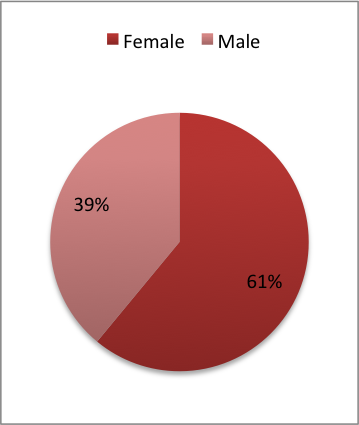
\includegraphics[width=0.7\linewidth]{./genderofconsumers}
\caption{Gender of Consumers (\%)}
\label{fig:genderofconsumers}
\end{figure}

\begin{figure}[tbph]
\centering
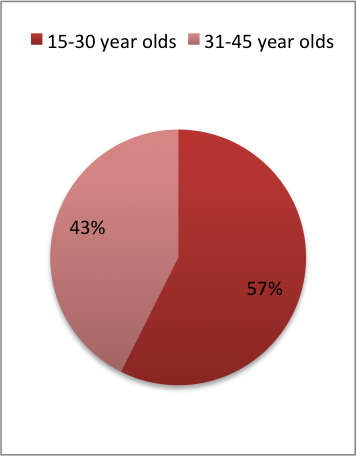
\includegraphics[width=0.7\linewidth]{./age}
\caption{Ages of Consumers (\%)}
\label{fig:agesofconsumers}
\end{figure}


The average frequency of Internet usage was 60 or more hours in a week. Furthermore, majority of respondents n= 79, 75\% have made an online purchase from Internet before. From collected these figures above, the Internet really has important effect on purchasing power in Vietnam.

To describe the number of using E-commerce times once week, Principal Components Analysis is conducted. As a result of the component analysis, rotated component matrix table is formed. From data of this table, the chart \textbf{(Fig. \ref{fig:ecfreq})} is drown to compare frequency of purchasing online goods from 75\% of 79 surveyed people. (Orange) Never/week; (Red) Less than 1 times/week; (Grey) From 1 to 3 times/week; (Green) From 4 to 7 times/week; (Moss Green) More than 7 times/ week.

\begin{figure}[tbph]
\centering
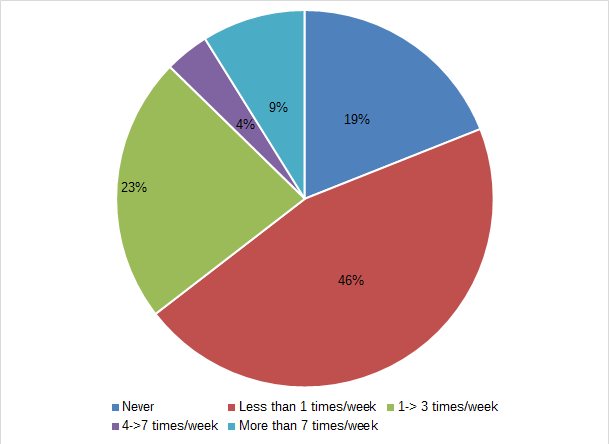
\includegraphics[width=0.7\linewidth]{./ecfreq}
\caption{Using E-commerce Frequency (\%)}
\label{fig:ecfreq}
\end{figure}


Besides, the author list out six regular activities of E-commerce user which are; (Grey) Use; (Red) No use; (1) Finding product information; (2) Using ATM; (3) Using International Cards; (4) Selling/Buying goods; (5) Buying courses/ Studying online; (6) Buying games/software; (7) Owning an online shop to evaluate utility of E-commerce to consumers. \textbf{(Fig. \ref{fig:ecactivities})}

\begin{figure}[tbph]
\centering
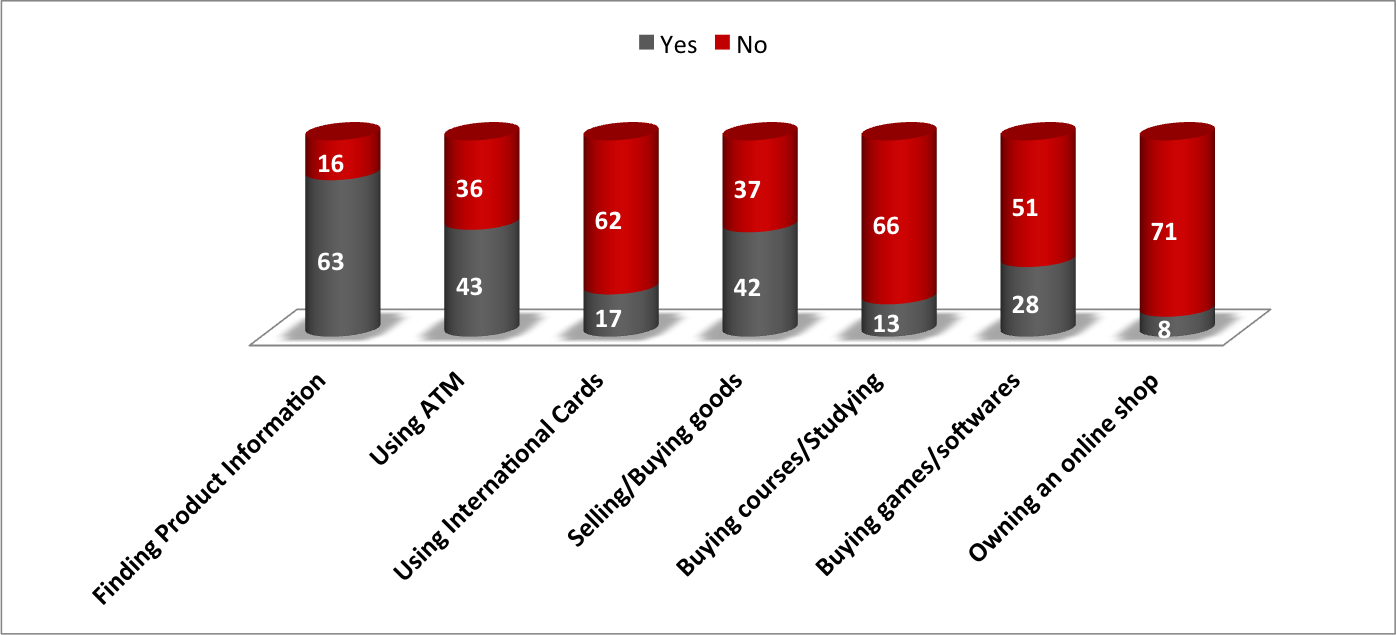
\includegraphics[width=0.7\linewidth]{./ecactivities}
\caption{Activities in E-commerce (person)}
\label{fig:ecactivities}
\end{figure}



With 90 people, who do not have knowledge about E-commerce, the authors introduce what is E-commerce and explain how to purchase online goods. After that, they are participated in a trial test to check their satisfactions about purchasing online goods. \textbf{(Fig. \ref{fig:satisfaction})}

\begin{figure}[tbph]
\centering
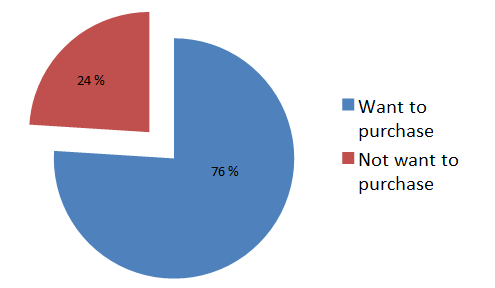
\includegraphics[width=0.7\linewidth]{./satisfaction}
\caption{Satisfaction of Consumers (person)}
\label{fig:satisfaction}
\end{figure}






\section{Conclusion} \label{conclusion}
When the potential is mentioned, people tend to think about the potential of the existing factors and forget that of the promising factors. However, from the results, the authors succeed in coming to two conclusions relating to both kinds of factors.

\begin{itemize}
\item The first conclusion involves those who do not have the chances to get access to the Internet. They are representative of the promising factors. However, the lack of knowledge about the Internet does not prevent them from being aware of and using E-commerce. After gain enough knowledge and have enough facilities, they start to use E-commerce. More than a half of them are willing to use E-commerce. In the future, they soon adapt to E-commerce, the new kind of purchasing goods. They are one of the most important sectors in E-commercial industry. E-commerce should be introduced and approach these factors.
\item In the second conclusion, the existing factors are proven. They are those who live in the urban area such as Ho Chi Minh City or Hanoi. They have the opportunities to get access to the Internet. They go online everyday and have time to get all the benefits the Internet brings to. Therefore, E-commerce is familiar with them. On the contrary, they said that they do not use E-commerce weekly. The reason is that they are not aware of the activities of the E-commerce. They use E-commerce without knowing it. That comes to the conclusion that these existing factors still have the potential for E-commerce. The E-commerce business should understand these factors and include them into the E-commerce. They extend the sector of E-commerce in the economy of Vietnam.

\end{itemize}




% conference papers do not normally have an appendix


% use section* for acknowledgement
\section*{Acknowledgment}


The authors would like to thank...





% trigger a \newpage just before the given reference
% number - used to balance the columns on the last page
% adjust value as needed - may need to be readjusted if
% the document is modified later
%\IEEEtriggeratref{8}
% The "triggered" command can be changed if desired:
%\IEEEtriggercmd{\enlargethispage{-5in}}

% references section

% can use a bibliography generated by BibTeX as a .bbl file
% BibTeX documentation can be easily obtained at:
% http://www.ctan.org/tex-archive/biblio/bibtex/contrib/doc/
% The IEEEtran BibTeX style support page is at:
% http://www.michaelshell.org/tex/ieeetran/bibtex/
%\bibliographystyle{IEEEtran}
% argument is your BibTeX string definitions and bibliography database(s)
%\bibliography{IEEEabrv,../bib/paper}
%
% <OR> manually copy in the resultant .bbl file
% set second argument of \begin to the number of references
% (used to reserve space for the reference number labels box)

\bibliographystyle{IEEEtran}
\bibliography{Bibtex}




% that's all folks
\end{document}

%[4] http://www.vecita.gov.vn/home/en last access on
%(February 2, 2015 at 10:57 PM)

%[5] Google Online Shopper Study, present by Ms. Trư ơng
%Thanh Hà, 2014, Hà N ội

%Vietnam E-commerce and Information Technology
%Agency, Vietnam Mobile E-Commerce Report, 2014

%[3] Vietnam E-commerce and Information Technology
%Agency, Vietnam Vietnam E-Commerce Report, 2013

%Information and Communications Publishing House,
%Information and Data on information and Communication
%Technology, 2014, page 56

%@book{Information and Data on information and Communication Technology,
%author = {Information and Communications Publishing House},
%title = {Information and Data on information and Communication Technology},
%date = {2014},
%}
